\documentclass[10pt,a4paper]{article}

\usepackage[utf8]{inputenc}
\usepackage[T1]{fontenc}
\usepackage[ngerman]{babel}
\usepackage[default]{lato}
\usepackage[margin=0pt]{geometry}
\usepackage{enumitem}
\usepackage{graphicx}
\usepackage{hyperref}
\usepackage{tabularx}
\usepackage{xcolor}
\usepackage{array}
\usepackage{microtype}
\usepackage{tikz}
\usepackage{fontawesome5}

\renewcommand{\familydefault}{\sfdefault}
\pagestyle{empty}
\setlength{\parindent}{0pt}
\setlength{\fboxsep}{0pt}
\setlength{\topskip}{0pt}
\raggedbottom
\graphicspath{{../assets/}{assets/}}
\hypersetup{colorlinks=true,urlcolor=accent,pdfauthor={Dinesh Gangatharan},pdftitle={Softwarearchitekt - Dinesh Gangatharan}}

\definecolor{bannerbg}{HTML}{20242C}
\definecolor{sidebarbg}{HTML}{EDEEF0}
\definecolor{accent}{HTML}{14919B}
\definecolor{heading}{HTML}{20242C}
\definecolor{muted}{HTML}{5B6168}

\newlength{\bannerheight}
\setlength{\bannerheight}{2.5cm}
\newlength{\sidepad}
\setlength{\sidepad}{14pt}

\newcommand{\sideheading}[1]{\vspace{0.9em}{\setlength{\fboxsep}{5pt}\colorbox{accent}{\parbox{\dimexpr\linewidth-10pt\relax}{\color{white}\bfseries\small #1}}}\par\vspace{0.5em}}
\newcommand{\mainheading}[1]{\vspace{0.3em}{\color{heading}\bfseries\Large #1}\par\vspace{0.15em}{\color{accent}\rule{\linewidth}{1.2pt}}\vspace{0.25em}}

\newcommand{\job}[5]{%
  \noindent{\bfseries #2}\hfill{\color{accent}\bfseries\small #1}\hspace{0.5em}\raisebox{-0.14cm}{\includegraphics[height=0.42cm,keepaspectratio]{#5}}\par
  {\color{muted}\itshape #3 --- \faMapMarker\ #4}\par\vspace{0.15em}}

\newcommand{\compactlist}{\begin{itemize}[leftmargin=1.1em,itemsep=0.12em,topsep=0.18em,parsep=0pt]}

\newcommand{\jobgap}{\vspace{0.55em}}

\newcommand{\prodrow}[3]{\noindent\begin{minipage}[t]{0.16\linewidth}\includegraphics[width=\linewidth]{#1}\end{minipage}\hfill\begin{minipage}[t]{0.80\linewidth}\href{#3}{#2}\end{minipage}\par\vspace{0.25em}}

\begin{document}
\noindent\colorbox{bannerbg}{%
  \parbox[t][\bannerheight][c]{\paperwidth}{%
    \hspace{0.9cm}\begin{minipage}[t]{\dimexpr\paperwidth-1.8cm\relax}
      {\fontsize{27}{30}\selectfont\bfseries\color{white} Dinesh Gangatharan}\par
      \vspace{0.15em}
      {\Large\color{accent} Senior Software Engineer / Softwarearchitekt}
    \end{minipage}%
  }%
}\par
\noindent
\begin{minipage}[t][\dimexpr\paperheight-\bannerheight\relax][t]{0.27\paperwidth}
  \colorbox{sidebarbg}{%
    \parbox[t][\dimexpr\paperheight-\bannerheight\relax][t]{\dimexpr\linewidth-2\sidepad\relax}{%
      \hspace{\sidepad}\begin{minipage}[t][\dimexpr\paperheight-\bannerheight\relax][t]{\dimexpr\linewidth-2\sidepad\relax}
      \setlength{\parskip}{0.25em}
      \vspace{0.6cm}
      \begin{center}
        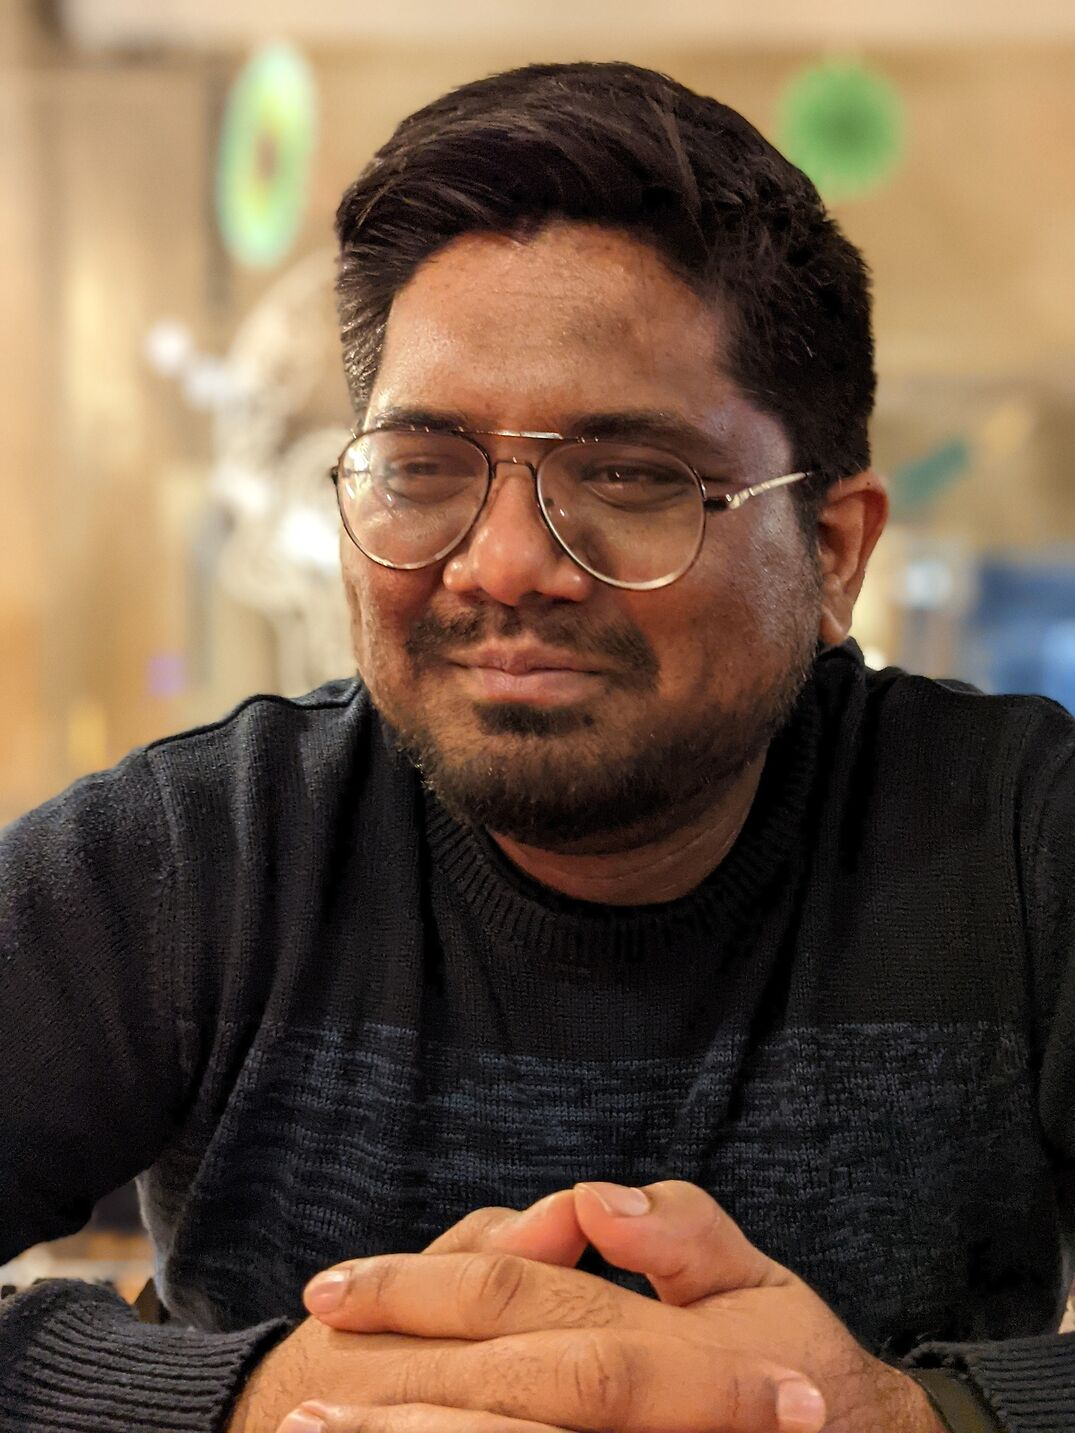
\includegraphics[width=3.4cm,keepaspectratio]{dinesh.jpeg}
      \end{center}
      \vfill
      \sideheading{SCHWERPUNKTE}
      \small Softwarearchitektur\par
      Mobile Entwicklung\par
      Kotlin Multiplatform\par
      CI/CD \& Gradle\par
      Backend-Integration

      \vfill
      \sideheading{ZERTIFIZIERUNG}
      \noindent\begin{minipage}[t]{0.20\linewidth}
\includegraphics[width=\linewidth]{isaqb_badge.png}\end{minipage}\hfill\begin{minipage}[t]{0.76\linewidth}\hyphenpenalty=10000\exhyphenpenalty=10000\href{https://www.credly.com/badges/7d95218f-8be4-455a-950c-c17663d5b9e9}{\textbf{iSAQB -- CPSA-F}}\par\footnotesize Certified Professional, Software Architecture\end{minipage}

      \vfill
      \sideheading{PRODUKTE}
      \small
      \prodrow{erezept.png}{E-Rezept}{https://play.google.com/store/apps/details?id=de.gematik.ti.erp.app}
      \prodrow{barmer.png}{Barmer eCare}{https://play.google.com/store/apps/details?id=de.barmer.ecare}
      \prodrow{rewe.png}{REWE}{https://play.google.com/store/apps/details?id=de.rewe.app.mobile}
      \prodrow{authada.png}{AUTHADA}{https://play.google.com/store/apps/details?id=de.authada.id}

      \vfill
      \sideheading{KOMPETENZEN}
      \small\raggedright
      \begin{itemize}[leftmargin=1.1em,itemsep=0.12em,topsep=0pt,parsep=0pt]
        \item Softwarearchitektur
        \item Zero Trust (ZETA)
        \item Kotlin Multiplatform (KMP)
        \item FHIR \& VZD
        \item CI/CD (Jenkins / Actions)
        \item Clean Architecture
      \end{itemize}

      \vfill
      \sideheading{LINKS}
      \footnotesize \mbox{\faGithub\ \href{https://github.com/dineshvg}{github.com/dineshvg}}\par
      \mbox{\faLinkedin\ \href{https://www.linkedin.com/in/dineshvg2310/}{linkedin.com/in/dineshvg2310}}

      \vfill
      \footnotesize \faEnvelope\ \href{mailto:dineshvg1023@gmail.com}{dineshvg1023@gmail.com}\par
      \faPhone\ +49 176 41637879\par
      \faMapMarker\ Stuttgart, Deutschland
      \vspace{0.6cm}
      \end{minipage}\hspace{\sidepad}%
  }
  }
\end{minipage}%
\begin{minipage}[t][\dimexpr\paperheight-\bannerheight\relax][t]{0.73\paperwidth}
  \hspace{0.75cm}\begin{minipage}[t][\dimexpr\paperheight-\bannerheight\relax][t]{\dimexpr\linewidth-1.5cm}
    \vspace{0.6cm}
    {\small\color{muted} Softwarearchitekt und Lead Android Developer für sichere Gesundheitssysteme, Kotlin Multiplatform, skalierbare Mobile-Architektur und automatisierte Auslieferung.}

    \vspace{0.9em}
    \mainheading{Berufserfahrung}

    \job{seit Feb. 2026}{gematik GmbH}{Softwarearchitekt}{Remote (Berlin)}{gematik-logo.png}
    \compactlist
      \item Lead Android Developer und Architekt der E-Rezept-App (Android, über 2~Mio. aktive Nutzer).
      \item Architektur des mobilen PoPP-Ökosystems (Proof of Patient Presence) und des KMP-SDK inkl. Zero Trust (ZETA) und NFC-Smartcard (PACE).
      \item Push-Gateway-Integration für sicheres Ende-zu-Ende-Routing von Push-Nachrichten und App-ID-Validierung in der TI.
      \item Konzeption der App-zu-App-Authentifizierung und eines lokalen Mock-IDP mit PKCE (RFC~7636) für Partnertests.
    \end{itemize}
    \jobgap

    \job{Sept. 2023 -- Jan. 2026}{gematik GmbH}{Lead Developer}{Remote (Berlin)}{gematik-logo.png}
    \compactlist
      \item Verantwortung für die E-Rezept-App (Android) und die FHIR-VZD-Backend-Dienste.
      \item Neuimplementierung des FHIR-Parsings (Kotlinx Serialization), Migration auf eine Multi-Modul-Architektur; CI/CD mit wiederverwendbaren Gradle-Plugins.
      \item Teamleitung, Mentoring und Koordination monatlicher Releases; Verbesserung der App-Bewertung von 2,0 auf 4,2.
    \end{itemize}
    \jobgap

    \job{Jan. 2022 -- Aug. 2023}{IBM iX DACH}{Senior-Entwickler}{Remote (Berlin)}{ibm-logo.png}
    \compactlist
      \item Entwicklung des digitalen Mutterpasses; Leitung einer Flutter-Initiative zur Zeiterfassung inkl. Python/Django-Backend.
      \item Plattformübergreifende Entwicklung mit Kotlin Multiplatform und SwiftUI, eng abgestimmt mit dem iOS-Team.
    \end{itemize}
    \jobgap

    \job{Juli 2019 -- Dez. 2021}{REWE Digital GmbH}{Softwareentwickler}{Köln}{rewe-logo.png}
    \compactlist
      \item Umsetzung von Full-Stack-Features mit Android SDK, Kotlin, TypeScript, Node.js, REST, Firebase und automatisierten Tests.
      \item Entwurf skalierbarer Architekturen mit MVVM, MVP und MVI.
    \end{itemize}
    \jobgap

    \job{Nov. 2016 -- Juni 2019}{AUTHADA GmbH}{Softwareentwickler}{Darmstadt}{authada-logo.jpg}
    \compactlist
      \item Entwicklung der Zertifizierungsfunktionen der Android-App.
      \item Migration von Java-Code nach Kotlin gemäß Clean-Code-Prinzipien und MVP.
    \end{itemize}

    \mainheading{Eigene Projekte}
    {\footnotesize
    \begin{itemize}[leftmargin=1.1em,itemsep=0.12em,topsep=0pt,parsep=0pt]
      \item \textbf{\href{https://github.com/dineshvg/health-plan-app}{Health plan $\rightarrow$ app}} (2026, Open Source): KI-Agenten-Skill (Claude Code), der aus Gesundheitszielen Pläne, einen Google-Sheets-Tracker und eine Offline-first-PWA erstellt; Privacy by Design, Playwright-Tests.
      \item \textbf{MCP-Server für KI-gestützte App-Tests} (2026): Kotlin-Multiplatform-MCP-Server, mit dem KI-Agenten Android-Apps per Prompt auf echten Geräten testen.
    \end{itemize}}

    \begin{minipage}[t]{0.48\linewidth}
      \mainheading{Ausbildung}
      \noindent\begin{minipage}[t]{0.76\linewidth}
        \raggedright{\bfseries M.Sc. Elektro- und Informationstechnik}\par
        {\small TU Darmstadt \hfill 2014--2017}
      \end{minipage}\hfill\raisebox{-0.3cm}{
\includegraphics[height=0.8cm,keepaspectratio]{tud.png}}\par\vspace{0.35em}
      \noindent\begin{minipage}[t]{0.76\linewidth}
        \raggedright{\bfseries B.E. Elektrotechnik}\par
        {\small Anna University \hfill 2006--2010}
      \end{minipage}\hfill\raisebox{-0.3cm}{
\includegraphics[height=0.8cm,keepaspectratio]{anna_univ_logo.png}}
    \end{minipage}\hfill
    \begin{minipage}[t]{0.48\linewidth}
      \mainheading{Publikationen}
      \footnotesize
      \begin{itemize}[leftmargin=1.1em,itemsep=0.3em,topsep=0pt,parsep=0pt]
        \item \href{https://www.researchgate.net/publication/320165052_Exercise_Monitoring_On_Consumer_Smart_Phones_Using_Ultrasonic_Sensing}{Exercise Monitoring on Consumer Smartphones Using Ultrasonic Sensing} (2017)
        \item \href{https://www.researchgate.net/publication/324942766_Fitness_Activity_Recognition_on_Smartphones_Using_Doppler_Measurements}{Fitness Activity Recognition on Smartphones Using Doppler Measurements} (2018)
      \end{itemize}
    \end{minipage}

    \vfill
    {\color{accent}\rule{\linewidth}{0.8pt}}\par\vspace{0.4em}
    {\centering\small\color{muted} \href{https://dineshvg.github.io}{dineshvg.github.io}\par}
    \vspace{0.5cm}
  \end{minipage}\hspace{0.75cm}
\end{minipage}
\end{document}
